\definecolor{codegreen}{rgb}{0,0.6,0}
\definecolor{codegray}{rgb}{0.5,0.5,0.5}
\definecolor{codepurple}{rgb}{0.58,0,0.82}
\definecolor{backcolour}{rgb}{0.95,0.95,0.92}
 
\lstdefinestyle{mystyle}{
    backgroundcolor=\color{backcolour},   
    commentstyle=\color{codegreen},
    keywordstyle=\color{magenta},
    numberstyle=\tiny\color{codegray},
    stringstyle=\color{codepurple},
    basicstyle=\footnotesize,
    breakatwhitespace=false,         
    breaklines=true,                 
    captionpos=b,                    
    keepspaces=true,                 
    numbers=left,                    
    numbersep=5pt,                  
    showspaces=false,                
    showstringspaces=false,
    showtabs=false,                  
    tabsize=2
}
 
\lstset{style=mystyle}


\section{Hadoop PageRank Cloud Computing}
\section*{Goal}
 
This assignment provides an illustration of PageRank algorithms and Hadoop. You
will then blend these applications by implementing a parallel version of
PageRank using the programming interfaces of the Hadoop MapReduce framework. 


\section*{Deliverables}
You are required to turn in the following items in a zip file
(username\_HadoopPageRank.zip) in this assignment: 

\begin{itemize}
\item The source code of Hadoop PageRank you implemented.
\item Technical report (username\_HadoopPageRank\_report.docx) that contains: 
\item The description of the main steps and data flow in your program. 
\item The output file (username\_HadoopPageRank\_output.txt) which contains the
  first 10 urls along with their ranks. 

\end{itemize}

\section*{Evaluation}
The point total for this exercise is 10, where the distribution is as follows:
\begin{itemize}
\item Completeness of your code and output (7 points)
\item Correctness of written report (3 points)
\end{itemize}

\section{What is PageRank?}
The web search engine is a typical distributed system on the Internet. It is
designed to search for information on the World Wide Web. The search results
are generally presented in a list of results and are often called hits.
PageRank is a well-known web graph ranking algorithm that helps Internet users
sort hits by their importance. 

PageRank calculates a numerical value for each element of a hyperlinked set of
webpages, which reflects the probability that a random surfer will access that
page. The process of PageRank can be understood as a Markov Chain which
requires iterative calculations to converge. An iteration of PageRank
calculates the new access probability for each webpage based on values
calculated in the previous iteration. The process will repeat until the number
of current iterations is bigger than predefined maximum iterations, or the
Euclidian distance between rank values in two subsequent iterations is less
than a predefined threshold that controls the accuracy of the output results. 

\begin{figure}[!htbp]
\centering
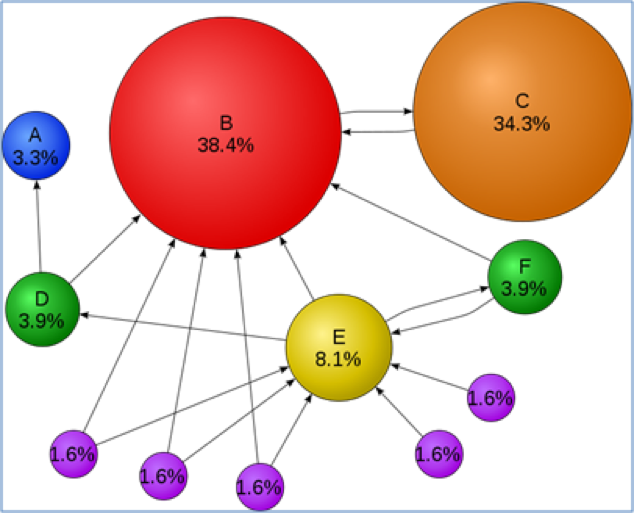
\includegraphics[width=8cm]{section/icloud/assignment/problems/project2/pagerankexample}
\caption{Mathematical PageRank for a simple network in Wikipedia}
\label{fig:pagerankexample}
\end{figure}

Figure~\ref{fig:pagerankexample} shows a web graph consisting of 11 vertices
{A, B, C, D, E, F, G1, G2, G3, G4, G5}. Each vertex refers to a unique webpage,
and the directed edge means there is one link from the source webpage to the
target webpage. The percentage on each vertex represents the rank value of each
webpage.

\subsection*{Notes}

You can implement a sequential PageRank that can run on desktops or laptops.
But when processing larger input data, like web graphs containing more than a
million webpages, you need to run the PageRank application in parallel so that
it can aggregate the computing power of multiple compute nodes. Currently, in
both industry and academia, the study of large-scale web or social graphs has
become increasingly popular. In one published paper, the job execution engines
that claim to support large-scale PageRank include: MPI, Hadoop, Dryad,
Twister, Pregel. 

\subsection*{Formula}

Equation~\ref{eq:pagerank} is the formula to calculate the rank value for each
webpage. We will learn this formula by applying it to the case in
Figure~\ref{fig:pagerankexample}. There are 11 webpages in
Figure~\ref{fig:pagerankexample}, which include: {A, B, C, D, E, F, G1, G2, G3,
G4, G5}. Assuming the probability distribution for a web surfer accessing all
these 11 pages in current iteration is \{PR(A), PR(B), PR(C), ... PR(G5)\},
then the probability for the surfer to access Page B in the next iteration is:
\\

$PR(B) = PR(D)/2 + PR(E)/3 + PR(F)/2 + PR(C) + PR(G1)/2 + PR(G2)/2 + PR(G3)/2 $\\


In a general case, the PageRank value for any page u can be expressed as:

\begin{equation}\label{eq:pagerank}
PR(u) = \sum_{v \in Set} \frac{PR(V)}{L(v)}
\end{equation}

The vertices seen in the right of the formula contain all the webpages that
point to target webpage 'u'. The L(v) refers to the out degree of each webpage
in the vertices set. The initial rank values of each webpage, like PR'(u), can
be any double value. After several iteration calculations, the rank values
converge to the stationary distribution regardless of what their initial values
are.

\subsection*{Damping factor}
The PageRank theory holds that even an imaginary surfer who is randomly
clicking on links will eventually stop clicking. The probability, at any step,
that the person will continue is a damping factor d. Various studies have
tested different damping factors, but it is generally assumed that the damping
factor will be around 0.85. The formula considering damping factor is shown in
Equation~\ref{eq:pagerankwithdf}. N refers to the total number of unique urls. 

\begin{equation}\label{eq:pagerankwithdf}
PR(u) = \frac{1-d}{N} + d * \sum_{v \in Set} \frac{PR(V)}{L(v)}
\end{equation}

\section*{Hadoop PageRank DataFlow}
In this exercise, we have provided a sketch code which contains three MapReduce
jobs for you to implement:

\begin{itemize}
\item CreateGraph (done): add one column, 'initial pagerank value', to the
  input pagerank adjacency matrix (AM). Then pass it to the PageRank program to
    calculate the pagerank values. 
\item PageRank (your implementation): take the transformed AM matrix and
  calculate pagerank values for all pages. 
\item Cleanup Results: remove the targetUrls column and output
  \textbf{(sourceUrl, pagerank value)} as the final result. 
\end{itemize}

The detail dataflow can be seen in Figure~\ref{fig:hadoopdataflow}. Part 1 and
Part 3 are given as full solutions in this pipeline; you will implement the 2nd
part of the PageRank program.

\begin{figure}[!htbp]
\centering

\includegraphics[width=10cm]{section/icloud/assignment/problems/project2/hadoopdataflow.png}
\caption{Hadoop PageRank dataflow}
\label{fig:hadoopdataflow}
\end{figure}

Normally for any Hadoop MapReduce program, input data is uploaded and stored in
the Hadoop Distributed File System (HDFS) before computation in order to
generate \textbf{(key, value)} pairs to the mapper. Initially, the PageRank
input data is stored in the format of adjacency matrix as a file(s) in the
local file system. Then it will be uploaded to the HDFS and distributed across
the compute nodes. Hadoop framework reads the application records from HDFS
with the InputFormat interface and generates \textbf{(key, value)} pair input
streams. Each Map function produces zero or more intermediate \textbf{(key,
value)} pairs by consuming one input (key, value) pair. For this PageRank
program, the map function applies the calculation $\frac{PR(v)}{L(V)}$ to each
\textbf{(key, value)} pair, where the key is the unique id or name of the
webpage and the value contains the current rank value of the webpage and its
out link information. Map tasks then generate intermediate (key, value) pairs,
whose value is the partial rank value of every webpage. Each reduce task
aggregates all the partial values of specific webpages by applying the provided
Equation~\ref{eq:pagerankwithdf}. The aggregated global rank values are written
back to HDFS, which in turn is used as input in the next set of iterations, if
any. "Hadoop - PageRank" in Figure~\ref{fig:hadoopdataflow} shows an example
for the PageRank data processing.


\section*{Code for Hadoop PageRank}

You need to complete two files in the provided pacakge inside
"indiana/cgl/hadoop/pagerank/": PageRankMap.java and PageRankReduce.java. Code
snapshots are shown below.

\lstinputlisting[language=Java]{section/icloud/assignment/problems/project2/PageRankMap.java}
\lstinputlisting[language=Java]{section/icloud/assignment/problems/project2/PageRankReducer.java}

\section*{Edit}
The sketch code is stored within the provided VirtualBox image. Use Eclipse or
linux text editor vi/vim to add your code.

\begin{lstlisting}[language=bash]
$ cd /root/MoocHomeworks/HadoopPageRank/
$ vim src/indiana/cgl/hadoop/pagerank/PageRankMap.java
$ vim src/indiana/cgl/hadoop/pagerank/PageRankReduce.java
\end{lstlisting}

\section*{Compile and run your code}
Use the one-click script compileAndExecHadoopPageRank.sh provided below.
Standard error messages such as compile errors, execution errors, etc. will be
redirected on the screen. Debug them based on the returned messages.

\begin{lstlisting}[language=bash]
$ cd /root/MoocHomeworks/HadoopPageRank/
# usage: ./compileAndExecHadoopPageRank.sh [PageRank Input File][Number of Urls][Number Of Iterations]
$ ./compileAndExecHadoopPageRank.sh PageRankDataGenerator/pagerank5000g50.input.0 5000 1
\end{lstlisting}

\section*{View the result}
The result is generated as /root/hbaseMoocAntProject/output/project2.txt. 
\begin{lstlisting}[language=bash]
$ cd /root/MoocHomeworks/HadoopPageRank/
$ cat output/*
\end{lstlisting}
